\documentclass[tikz,border=6pt]{standalone}
\usepackage[T1]{fontenc}
\usepackage{lmodern}
\usepackage{amsmath,amssymb}
\usetikzlibrary{arrows.meta,angles,quotes,calc,positioning}
\definecolor{axis}{HTML}{40515F}
\definecolor{grid}{HTML}{DDE4E8}
\definecolor{blue}{HTML}{3568D4}
\definecolor{coral}{HTML}{EF626C}
\definecolor{teal}{HTML}{2A9D8F}
\definecolor{gold}{HTML}{D89432}
\definecolor{purple}{HTML}{7357C8}
\tikzset{
  axisline/.style={axis, line width=.85pt, -{Stealth[length=3mm]}},
  guide/.style={axis!45, line width=.75pt, dashed},
  vector/.style={line width=1.5pt, -{Stealth[length=3mm]}},
  dot/.style={circle, fill=white, draw, line width=1.15pt, inner sep=2.15pt},
  label/.style={font=\large},
  smalllabel/.style={font=\normalsize}
}
\begin{document}

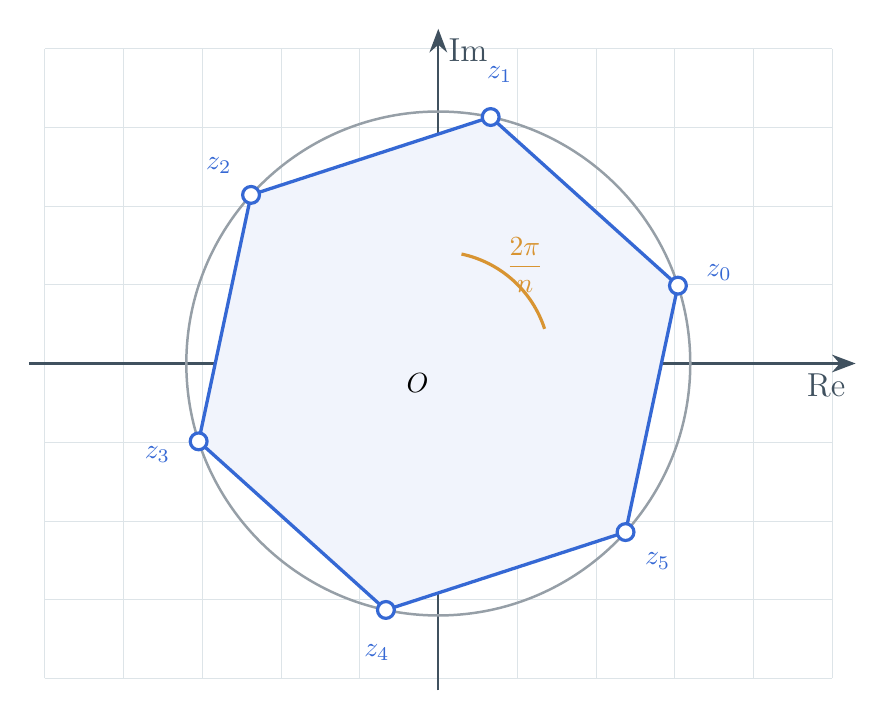
\begin{tikzpicture}[x=1cm,y=1cm]
  \draw[step=1cm,grid,very thin] (-5,-4) grid (5,4);
  \draw[axisline] (-5.2,0)--(5.3,0) node[below left,font=\large] {$\operatorname{Re}$};
  \draw[axisline] (0,-4.15)--(0,4.25) node[below right,font=\large] {$\operatorname{Im}$};
  \draw[axis!55,line width=.9pt] (0,0) circle[radius=3.2];
  \foreach \k in {0,...,5}{
    \coordinate (Z\k) at ({3.2*cos(18+60*\k)},{3.2*sin(18+60*\k)});
  }
  \draw[blue,line width=1.2pt,fill=blue!7] (Z0)--(Z1)--(Z2)--(Z3)--(Z4)--(Z5)--cycle;
  \foreach \k in {0,...,5}{
    \node[dot,draw=blue] at (Z\k) {};
    \node[smalllabel,blue] at ({3.75*cos(18+60*\k)},{3.75*sin(18+60*\k)}) {$z_{\k}$};
  }
  \draw[gold,line width=1.15pt] (1.35,0.44) arc[start angle=18,end angle=78,radius=1.42];
  \node[smalllabel,gold] at (1.1,1.25) {$\dfrac{2\pi}{n}$};
  \node[smalllabel,below left] at (0,0) {$O$};
\end{tikzpicture}
\end{document}
